% !TEX TS-program = pdflatex
% !TEX encoding = UTF-8 Unicode

% This is a simple template for a LaTeX document using the "article" class.
% See "book", "report", "letter" for other types of document.

\documentclass[11pt]{article} % use larger type; default would be 10pt

\usepackage[utf8]{inputenc} % set input encoding (not needed with XeLaTeX)

%%% Examples of Article customizations
% These packages are optional, depending whether you want the features they provide.
% See the LaTeX Companion or other references for full information.

%%% PAGE DIMENSIONS
\usepackage{geometry} % to change the page dimensions
\geometry{a4paper} % or letterpaper (US) or a5paper or....
% \geometry{margin=2in} % for example, change the margins to 2 inches all round
% \geometry{landscape} % set up the page for landscape
%   read geometry.pdf for detailed page layout information

\usepackage{graphicx} % support the \includegraphics command and options
\usepackage{datetime}
\usepackage{amssymb,amsmath} % For mathematical expressions  (Tillagd av Nai) 

%%% NEW COMMANDS
\renewcommand{\dateseparator}{-}
\newdateformat{mydate}{\THEYEAR \dateseparator0\THEMONTH \dateseparator \THEDAY} 
\renewcommand{\figurename}{Figur}

% \usepackage[parfill]{parskip} % Activate to begin paragraphs with an empty line rather than an indent

%%% PACKAGES
\usepackage{booktabs} % for much better looking tables
\usepackage{array} % for better arrays (eg matrices) in maths
\usepackage{paralist} % very flexible & customisable lists (eg. enumerate/itemize, etc.)
\usepackage{verbatim} % adds environment for commenting out blocks of text & for better verbatim
\usepackage{subfig} % make it possible to include more than one captioned figure/table in a single float
% These packages are all incorporated in the memoir class to one degree or another...

%%% HEADERS & FOOTERS
\usepackage{fancyhdr} % This should be set AFTER setting up the page geometry
\pagestyle{fancy} % options: empty , plain , fancy
\renewcommand{\headrulewidth}{0pt} % customise the layout...
\lhead{}\chead{}\rhead{}
\lfoot{}\cfoot{\thepage}\rfoot{}

%%% SECTION TITLE APPEARANCE
\usepackage{sectsty}
\allsectionsfont{\sffamily\mdseries\upshape} % (See the fntguide.pdf for font help)
% (This matches ConTeXt defaults)

%%% ToC (table of contents) APPEARANCE
\usepackage[nottoc,notlof,notlot]{tocbibind} % Put the bibliography in the ToC
\usepackage[titles,subfigure]{tocloft} % Alter the style of the Table of Contents
\renewcommand{\cftsecfont}{\rmfamily\mdseries\upshape}
\renewcommand{\cftsecpagefont}{\rmfamily\mdseries\upshape} % No bold!

%%% END Article customizations






%%% The "real" document content comes below...

\pagenumbering{gobble}
\title{Projektrapport Grupp 3 \\* 
CUURRLLInNNNGGG!\\*
TNM??? Modelleringsprojekt}
\author{Linnéa Mellblom\\*Linnea Malcherek\\* Julia Nilsson\\*Michael Nilsson\\*Linnéa Nåbo}
%\date{} % Activate to display a given date or no date (if empty),
         % otherwise the current date is printed 
\mydate


\begin{document}
\maketitle
\pagebreak
\pagenumbering{arabic}  

\section{Redogörelse för arbetet}

\subsection{Translation}

I beräkningarna av stenens rörelse har hänsyn tagits till tre påverkande friktionskrafter: Kraft i riktning motsatt stenens rörelseriktning, samt två krafter i ortogonal riktning mot denna \eqref{Ftot}. Dessa två krafter utgörs av friktionskrafterna i främre delen av stenen samt i den bakre delen. Differensen mellan dessa två krafter är vad som påverkar stenens curl. 
Stenens curl beror på att friktionen i den bakre delen av stenen är högre än den främre, på grund av de spår som den främre delen av stenen skapar i isen. REFERENS! 

 \begin{align}\label{Ftot}
 \bar{F_t}&=\bar{F_f}+\bar{F_b}+\bar{F}\\
 \bar{F_f}&<\bar{F_b}
 \end{align}

Translationen av stenen är en resulterande hastighetsvektor v, som består av hastigheten i rörelseriktningen samt av hastigheten i punkterna längs det ringformade band stenen roterar på. I beräkningarna har dessa förenklats till två hastighetsvektorer: en för den främsta punkten (p1)  på stenens band och en för den bakersta (p2),(Figur~\ref{fig:Translation}). 

\begin{figure}[ht!]
\centering
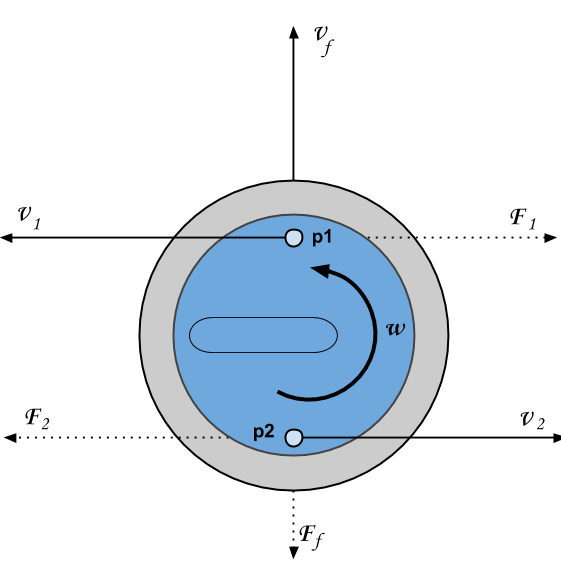
\includegraphics[width=80mm]{Translation.png}
\caption{Påverkan av stenens translation}
\label{fig:Translation}
\label{overflow}
\end{figure}

Beräkningen av hastigheterna i punkterna p1 och p2 beräknas i två steg. I första steget omvandlas stenens rotationshastighet till translationshastighet i riktningen i punkternas rotationsriktning \eqref{vsida_init}. 
 
\begin{align}\label{vsida_init}
 v_1 = v_1 = \omega r
 \end{align}

I det andra steget beräknas den påverkan som friktionen har på hastigheten i de två punkterna \eqref{Fsida1} \eqref{Fsida2}, där friktionen påverkas av hastigheten i punkten samt av en konstant c \eqref{mu} . 

 \begin{align}\label{Fsida1}
 F_1& = \mu_1 mg\\\label{Fsida2}
F_2& = \mu_2 mg\\\label{mu}
\mu&=\frac{c}{\sqrt{v}}
 \end{align}

Hastigheterna i de två punkterna blir därmed två hastighetsvektorer i motsatta riktningar där den ena är större än den andra och resultanten blir således den riktning åt vilken stenen curlar (Figur~\ref{fig:Translation}). 
Translationen av stenen i riktning framåt beräknas enligt Eulers stegmetod och med konstant friktionskoefficient. 

Den resulterande hastigheten består i beräkningarna således av tre komponenter  %\eqref{vtot}. 

 \begin{align}\label{vtot}
 &\bar{v}=\bar{v_f}+(\bar{v_1}+\bar{v_2})
 \end{align}

\subsection{Rotation}


%Stenen har även en roterande rörelse med en vinkelhastighet vars ursprungsvärde beräknas utifrån utslagshastigheten av %stenen.
%Vid utslaget antas att spelaren håller stenen så att handtaget pekar i en riktning 90 GRADER från riktning framåt antingen med %"inhand" eller "outhand" och släpper stenen med handtaget pekande rakt fram vid hoglinjen LITE BILDER PÅ BANAN. Detta %innebär att stenen roterar 90 GRADER under den tid det tar för spelaren att ta sig mellan hack och hog, vilket är direkt kopplat till %den angivna utslagshastigheten. 

\begin{align}%\label{vtot}
 angular_speed1 = pi / (2*t0); 
 \end{align}


 Den roterande rörelsen påverkas av friktionen mot isen. 

\subsection{Kollision}


 \begin{align} % &-tecknen gör att de alignar
% Position
 pos&=pos_n+\bar{v_n}\Delta t \\  %Oklar på hur man gör längre nedsänkningar än ett tecken (ex. n+1) 
% Speeds and velocities
 v&=v_n+a \Delta t \\ 
 \omega&=\omega_n+\alpha \Delta t  
 \end{align}

\subsection{Kollision}

För att kontrollera att en kollision sker beräknar vi avståndet mellan stenarnas position.

Hastigheten och riktningen av curlingstenarna efter en kollision beräknas med hjälp av de två stenarnas position och hastighetsvektorer. 

Kontroll av kollision
Inelastiskt
Delas upp i två komponenter, normal och tangent.




\section{Mål}



\begin{enumerate}
\item Här är en numrerad lista
\item Filtrera 
\item Kontrollera 
\item Göra 
\item Skapa 
\item Möjlighet 
\end{enumerate}


\pagebreak 



\subsection{Kravhantering}

Här är en sektion

\subsection{Principer och rutiner vid testning}

\subsubsection{Allmänt}
Här är en subsektion

\subsubsection{Rutiner för test}
Och en subsub!

Här är en onumrerad lista
\begin{itemize}
\item Olika
\item Att 
\item Att
\item Om 
\end{itemize}



Systemarkitekturen utgörs av ett Use-Case Diagram, och här kommer den automatiska referensen till den:   (Figure ~\ref{fig:Translation}).

\begin{figure}[ht!]
\centering
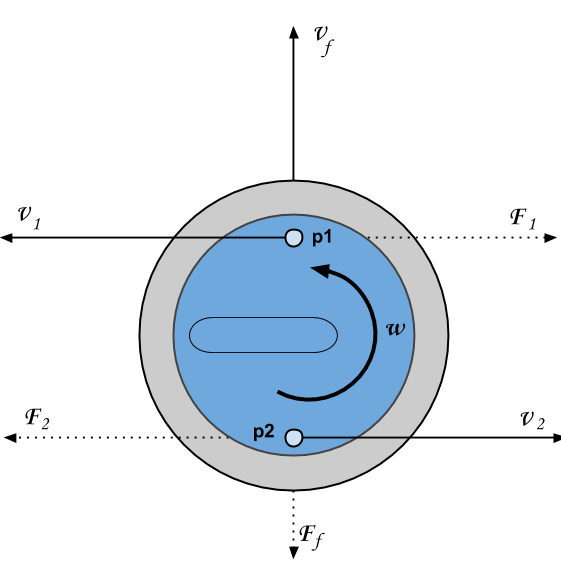
\includegraphics[width=80mm]{Translation.png}
\caption{Translation}
\label{fig:Translation}
\label{overflow}
\end{figure}


\pagebreak


\section{Projektmedlemmar}

Linnea Malcherek - projektledare och scrum master\\*
Julia Nilsson - kundkontakt och produktägare\\*
Linnéa Nåbo \\*
Lovisa Dahl\\*





\end{document}
